%XeLaTex+MakeIndex+BibTex
\documentclass[12pt]{article}
\usepackage{fontspec}
\usepackage{polyglossia}
\usepackage{geometry}
\usepackage{xcolor}
\usepackage{titlesec}
\usepackage{fancyhdr}
\usepackage{graphicx}
\usepackage{mathtools}
\graphicspath{{../plotting/figures/}}
\usepackage{hyperref} % Add hyperref package for clickable links
\usepackage{amsmath}
\usepackage{tabularx}
\usepackage{algorithm}
\usepackage{algorithmic}

\usepackage{float}
\usepackage{caption}
\usepackage{subcaption}

\usepackage[numbib]{tocbibind}

% Set the page margins
\geometry{a4paper,margin=2.54cm}

%\usepackage{kmath,kerkis} % The order of the packages matters; kmath changes the default text font
%\usepackage[T1]{fontenc}

% Set the font to Kerkis
\setmainfont{Calibri}


\usepackage{matlab-prettifier}
\newfontfamily\greekfonttt[Script=Greek]{Calibri}

% Define colors
\definecolor{myblue}{RGB}{0, 51, 102}
\definecolor{mygray}{RGB}{150,150,150}
\definecolor{mybg}{RGB}{230,230,230}

% Set line spacing
\usepackage{setspace}  % Required for custom line spacing
\setstretch{1.15}      % Set custom line spacing

% Set section title formatting
\titleformat{\section}
  {\normalfont\Large\bfseries\color{myblue}}
  {\thesection}{1em}{}
%\titleformat{\subsection}
%  {\normalfont\Large\bfseries\color{myblue}}
%  {\thesubsection}{1em}{}

\setmainlanguage{greek}
\setotherlanguage{english}

% Define header and footer
\pagestyle{fancy}
\fancyhf{}
\lhead{Βαπόρης - Ντελόπουλος}
\rhead{Απλοποιημένος κωδικοποιητής/αποκωδικοποιητής AAC}
\cfoot{\thepage}


\begin{document}
\begin{titlepage}
\newgeometry{margin=2.54cm}
\centering
\begin{figure}[H]
\centering
\includegraphics[width=0.8\textwidth]{banner-horizontal-black-en.png}\par % Image on top of title
\end{figure}
%\textcolor{black}{\large \bfseries Αριστοτέλειο Πανεπιστήμιο Θεσσαλονίκης\\}\par
\vspace{18pt}
\textcolor{black}{\Large \bfseries Τμήμα Ηλεκτρολόγων Μηχανικών\\ και Μηχανικών Υπολογιστών\\}\par
\vspace{1cm}
\vfill
\textcolor{black}{\Large \bfseries Απλοποιημένος κωδικοποιητής/αποκωδικοποιητής AAC}\par
\vspace{12pt}
\textcolor{black}{\large \bfseries Συστήματα Πολυμέσων - Ομαδική Εργασία}\par

\vspace{0.5cm} % Adjust vertical spacing here
\vfill
\newcolumntype{L}{>{\raggedright\arraybackslash}X}%
\newcolumntype{R}{>{\raggedleft\arraybackslash}X}%
{\large
\def\arraystretch{1.3}
\begin{tabularx}{\textwidth}{ R|L }
\textbf{Βαπόρης Δημήτριος}          & ΑΕΜ 10625\\
\textbf{Ντελόπουλος Εμμανουήλ}      & ΑΕΜ 10693\\
\textbf{Εργαστηριακός Υπεύθυνος}    & Αλέτρας Δημήτριος\\
\textbf{Υπεύθυνος Καθηγητής}        & Ντελόπουλος Αναστάσιος\\
\end{tabularx}
}
\vspace{0.5cm}
\vfill
\textcolor{black}{\large \bfseries Χειμερινό Εξάμηνο 2025-2026}\par
\end{titlepage}
\restoregeometry

\tableofcontents % Table of Contents
\clearpage

\section{Εισαγωγή}

\section{Επίπεδο 3}
\begin{figure}[H]
  \centering
  \includegraphics[width=0.8\textwidth]{compression_rates_vs_bias.pdf}
  \caption{Σχέση μεταξύ COMPRESSION\_BIAS και Compression Rate}
  \label{fig:compression_rates_vs_bias}
\end{figure}

\begin{figure}[H]
  \centering
  \includegraphics[width=0.8\textwidth]{snr_vs_bias.pdf}
  \caption{Σχέση μεταξύ COMPRESSION\_BIAS και SNR}
  \label{fig:snr_vs_bias}
\end{figure}

\begin{figure}[H]
  \centering
  \includegraphics[width=0.8\textwidth]{waveform_zoom_comparison.pdf}
  \caption{Σύγκριση κυματομορφών (COMPRESSION\_BIAS=30)}
  \label{fig:waveform_zoom_comparison}
\end{figure}
\begin{figure}[H]
  \centering
  \includegraphics[width=0.8\textwidth]{frame_type_distribution.pdf}
  \caption{Κατανομή τύπων πλαισίων (COMPRESSION\_BIAS=30)}
  \label{fig:frame_types_distribution}
\end{figure}

\begin{figure}[H]
  \centering
  \includegraphics[width=0.8\textwidth]{error_signal_over_time.pdf}
  \caption{Σφάλμα σήματος σε σχέση με τον χρόνο (COMPRESSION\_BIAS=30)}
  \label{fig:error_signal_over_time}
\end{figure}

\begin{figure}[H]
  \centering
  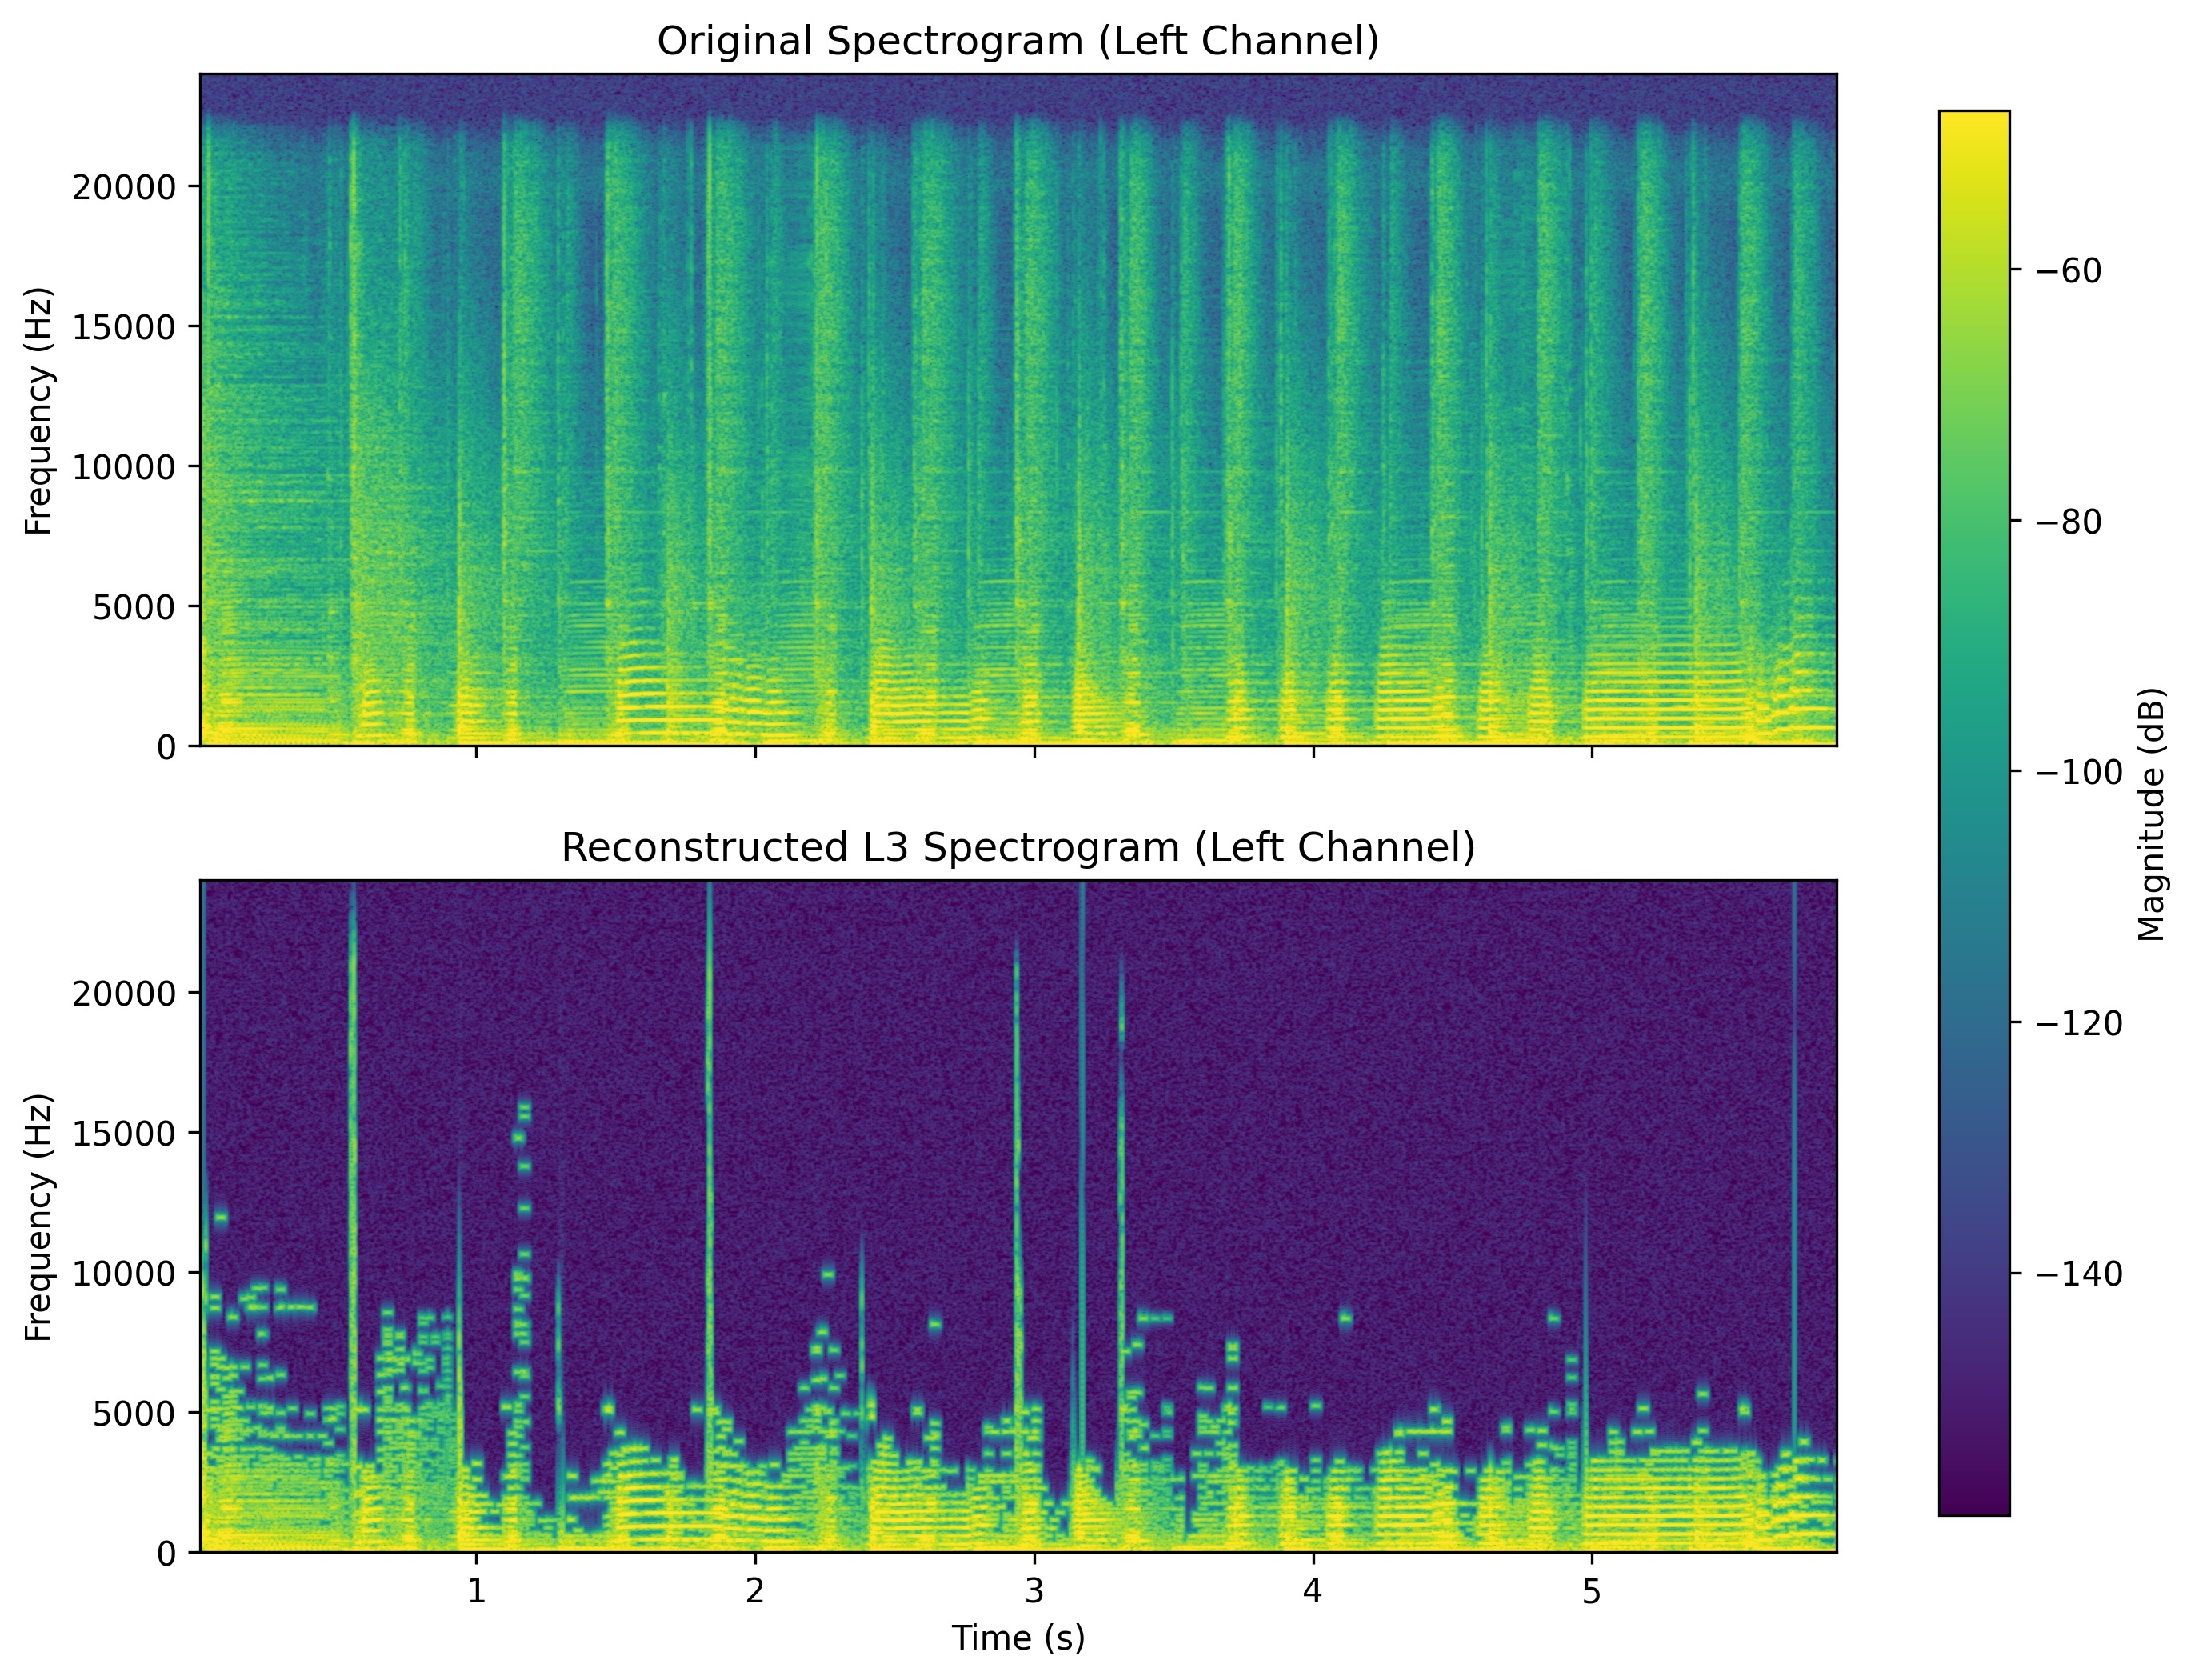
\includegraphics[width=0.8\textwidth]{spectrogram_comparison.png}
  \caption{Σύγκριση φασματογράμματος (COMPRESSION\_BIAS=30)}
  \label{fig:spectrogram_comparison}
\end{figure}

\clearpage
\listoffigures
\end{document}